\documentclass{article}
\usepackage[utf8]{inputenc}
\usepackage{blindtext}
\usepackage[T1]{fontenc}
\usepackage{amsmath}
\usepackage{amsfonts}
\usepackage{latexsym}
\usepackage{times}
\usepackage[T1]{fontenc} 
\usepackage{graphicx}
\usepackage{listings}
\usepackage{color}
\usepackage{tikz}
\definecolor{dkgreen}{rgb}{0,0.6,0}
\definecolor{gray}{rgb}{0.5,0.5,0.5}
\definecolor{mauve}{rgb}{0.58,0,0.82}
\usepackage[T1]{fontenc}
\usepackage[english,swedish]{babel}
\usepackage[utf8]{inputenc}
\usepackage[a3paper,twoside]{geometry}
\geometry{left=5cm,right=4cm,top=5cm,bottom=6cm}
\usepackage{sectsty} 
\usepackage{graphicx}
\usepackage[export]{adjustbox}
 \sectionfont{\fontsize{12}{14}\selectfont}
\subsectionfont{\fontsize{10}{14}\selectfont}
\subsubsectionfont{\fontsize{10}{14}\selectfont}
\newcommand{\summation}[2]{\sum_{i=0}^{#1}{#2}_i}





\begin{document}

\title{\textbf{\LaTeX\  \\*
The Benefits of Virtual Reality and Augmented Reality in Education }}
\author{Rashed Qazizada\thanks{ra222ah@student.lnu.se}}

\maketitle
\newpage
\begin{abstract}
    Here you can write you abstract.
    
\end{abstract}


 \newpage
\selectlanguage{english}
\tableofcontents

\newpage
 


\section{Assignment}


\subsection{Assignment 1}

\textbf{This text is in bold.}\\
\textit{This text is in Italics.}\\
This is a simple example, {\tiny this will show different font sizes} and also \textsc{different font styles}.
\subsection{Assignment 2}

\begin{equation*}
    \frac{\sin mx}{\sin x}=(-4)^{(m-1)/2} \prod_{j=1}^{(m-1)/2} 
    \left( \sin^2x - sin^2\frac{2\pi j}{m} \right)
    \end{equation*}

Equation can be also written as follow $f_n = f_{n-1} + f_{n-2} $


\subsection{Assignment 3 \& 4}

\selectlanguage{english}

\begin{table}[htbp]
	\centering
	\begin{tabular}{l l l r@{.}l}
		\hline 
		& & \multicolumn{3}{c}{\textbf{World Record}} \\ 
		\cline{3-5}
		\bfseries{Name} & \bfseries{Country} & \bfseries{Event} & \multicolumn{2}{c}{\bfseries{Result}}				 \\ 
		\hline Anna-Karin Kammerling & Sweden & 50 m butterfly & 25&57 \\ 
		Wilson Kipketer & Denmark & 800 m & 2:11&96 \\ 
		Jan 
		\v{Z}elezný & Czech Republic & javelin throw & 98&5 \\ 
		Sergei Bubka & Ukraine & pole vault & 6&14 \\ 
		\hline 
	\end{tabular}  
	\caption{World Record and Results} 
	\label{Table1} 
	\end{table} 
	The table shows the world record and results (\ref{Table1})
	\footnote{Here where you can write your footnote}
	
	
 
	
\subsection*{Assignment 5}
\begin{figure}[h]
\begin{center} 
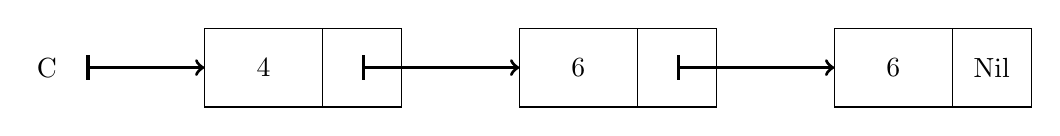
\begin{tikzpicture} 
\node at(0,0.5) {C};
    \node at(2.75 ,0.5) {4};
    \node at(6.75,0.5) {6};
    \node at(12 ,0.5) {Nil};
    \node at(10.75,0.5) {6};
    \draw [very thick][|->] (0.5,0.5) -- (2,0.5);
    \draw (2,0) rectangle (3.5,1);
    \draw (3.5,0) rectangle (4.5,1);
     \draw [very thick][|->] (4,0.5) -- (6,0.5);
     \draw (6,0) rectangle (7.5,1);
     \draw (7.5,0) rectangle (8.5,1);
     \draw [very thick][|->] (8,0.5) -- (10,0.5);
     \draw (10,0) rectangle (11.5,1);
     \draw (11.5,0) rectangle (12.5,1);
     
\end{tikzpicture} 
\end{center}
\caption{ Shows TikZ Typeset }
	\label{f:tikz}
\end{figure}
Here figure \ref{f:tikz} shows the Assignment 5.


\subsection{Assignment 6 \& 7\\A brilliant way to get children running for fun!}
 
\begin{figure}[h]
    \centering
    
    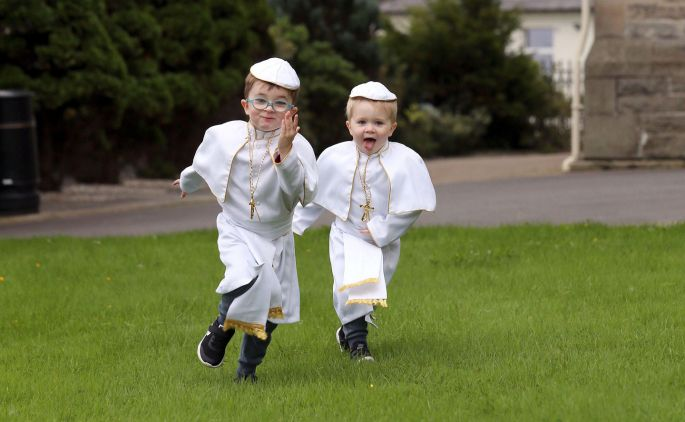
\includegraphics[width=0.8\textwidth, center]{image.jpg}
    \caption{Greek Orthodox Church}
    \label{fig:my_label}
\end{figure}

The figure \ref{fig:my_label} shows a perfectly competitive children.
  
\subsection{Assignment 8}
\begin{flushleft}
    $x^{n^2} + y^{n + 1} = z^n $  Right brace and a dollar character were missing.
\emph{The Johansson Brothers \& Son.}
(b)emph was misspelled with an extra h and backslash was missing before the et-character. \LaTeX\ is case sensitive.\\
(c) .. end of a paragraph. \\*
A new paragraph ...

Additional line-breaking commands(two backslashes and an asterisk)\\
lines breaks (two backslashes without asterisk)
\end{flushleft}




\subsection{Assignment 9}

\begin{lstlisting}
Scanner scan = new Scanner(System.in);
		System.out.print("Enter a postive integers: ");
		int userInput = scan.nextInt();
		int zero = 0, odd =0, even =0; // Initialising zero,odd,and Even.
		
		while (userInput > 0) {			//step1 10023>0 step3 1002%10=2 step5 100%10=0
			int digit = userInput % 10;		
			if (digit == 0) {
				zero++; 
			} else if (digit % 2 == 0) {	//step4 2%2=0
				even++; 
			} else {
				odd++; 
			}
			userInput = userInput / 10;	// step2 10023=1002 step6 10/10=1
		}
		System.out.println("Zeros: " + zero);
		System.out.println("Odds: " + odd);
		System.out.println("Evens: " + even);
		scan.close();
	}

}
\end{lstlisting}

\subsection*{Assignment 10}
\begin{equation}
\summation{n}{\alpha}
\hspace{1cm}
\summation{10}{\gamma}
\hspace{1cm}
\summation{50}{\beta}
\end{equation}

\subsection{Assignment 11}
A comment can be written here\cite{Peter J.Cameron} ,  or another text can be written here as well\cite{Patrick Morton}.



\begin{thebibliography}{2}
\bibitem[1]{Peter J.Cameron}P.J.Cameron, \emph{Permutations Groups}. Cambridge : Cambridge University Press, 1999.

\bibitem[2]{Patrick Morton} P. Morton, "Periods of Maps or Irreducible Polynomials over Finite Field", \emph{Finite Fields and their Applications (Finite Fields Appl.)}, vol. 3, pp. 11-24, 1997.
\end{thebibliography}


\section{Template for my final report}
\subsection{Discussion}

\subsection{Conclusion}





\end{document}